
%(BEGIN_QUESTION)
% Copyright 2006, Tony R. Kuphaldt, released under the Creative Commons Attribution License (v 1.0)
% This means you may do almost anything with this work of mine, so long as you give me proper credit

Control valves used in pneumatic and hydraulic fluid power systems often take the form of a {\it spool} mechanism, and the fluid power schematic symbols for these spool valves are quite unlike that of valve symbols in P\&IDs and loop diagrams:

$$\includegraphics[width=15.5cm]{i00753x01.eps}$$

Explain what these symbols represent, and how they are to be interpreted.  Also, comment on the construction of a spool valve.

\underbar{file i00753}
%(END_QUESTION)





%(BEGIN_ANSWER)

The symbols show each valve's ``normal'' (unactuated) position.  To understand what happens when the valve is actuated, you must visualize the boxes sliding over into alignment with the inlet/outlet pipes, like this:

$$\includegraphics[width=15.5cm]{i00753x02.eps}$$

The same holds for the reversing valve, except that it has three positions:

$$\includegraphics[width=15.5cm]{i00753x03.eps}$$

%(END_ANSWER)





%(BEGIN_NOTES)

Directional valves used in hydraulic systems often use these labels to designate ports:

\begin{itemize}
\item{} P = Pressure source (from pump)
\item{} T = Return to tank (reservoir)
\item{} 1 = To one side of cylinder
\item{} 2 = To other side of cylinder
\end{itemize}

Sometimes, though, the letters ``A'' and ``B'' are used instead of the numbers ``1'' and ``2'' to designate the hydraulic cylinder connections.

%INDEX% Mechanics, fluid power systems: spool valve symbols

%(END_NOTES)


